\section{Libvina: A template library}\label{sec:lib}
We implement a prototype template library, libvina,  to demonstrate
our approach. Libvina consists of 3 components: (1) View class, a representation of underlying containers such as vector or matrix. (2) Building block class,
provide basic executions of tasks on multicores (3) TF class, each one
represents a parallel pattern. 

\subsection{View class}
To leverage static information, libvina need to
associate template parameters with ADTs' parameters. For example, 
Matrix class cantains 3 template paramters: type, the number of
row, the number of column. A definition of Matrix is at line 26 of
List 1. A \emph{View} is a class representing the subset of containers' data. There
are two kinds of views: ReadView and WriteView. Variants like
ViewMTs serve for multithreaded programs. 
A ReadView is read-only. A WriteView has interfaces to write  as
well. ViewMTs contains signals, which are copied across multiple
threads. All operations of ViewMTs are blocking until signals are sent
by other views.

Fig.~\ref{fig:view} depicts relationship of views in
libvina. Concrete lines represent implicit conversion in C++, while
dashed lines are explicit function calls to complete conversion. Text
in edges are constraints for conversions. Line 30$\sim$32 of
List 1 generate subviews by calling functions. Shadow region is
another thread space.
%The only approach to communicate with other
%threads is through a special kind of view called \emph{ViewMT}.  

The design of view class has two purposes. 1) The classes are type-safed.
Because template instantiation is not visible for programmers, our
source transformations by templates could introduce subtle errors. We
expect compilers complain explicitly when unintentional
transformations happen. 2) View classes hide communication details. 
Implementations have choice to optimize data movement according to
architectures. Shared memory systems~\cite{larrabee} and communication-exposed multicores~\cite{cellbe, imagine} usually have different strategies to perform
the operations.

\begin{figure}
%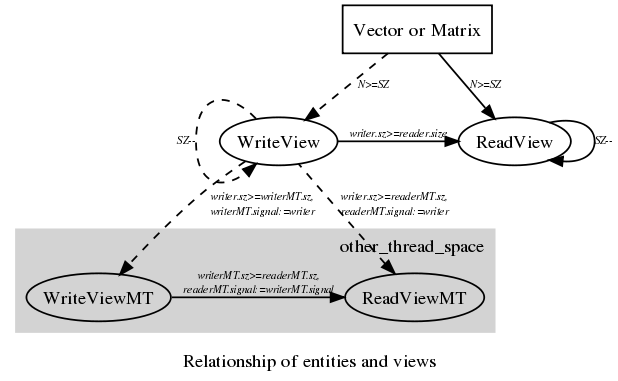
\includegraphics[width=3.6in,height=3.0in]{../relationship_views}
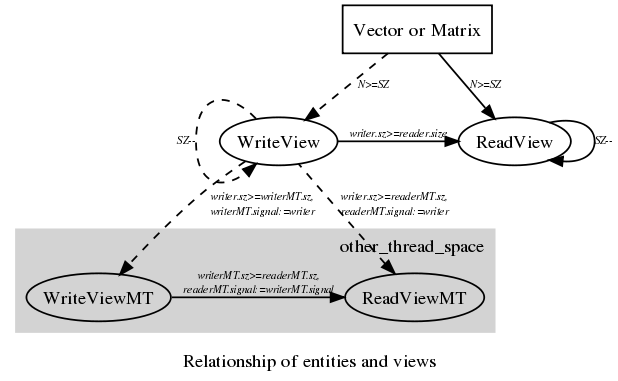
\includegraphics[width=3.6in, height=2.5in]{../relationship_views}
\caption{View classes in libvina: A view represents subset of
  underlying constrainers. A ReadView is read-only. A WriteView
  can write back as well. Edges are  conversions. A concrete line is implicit conversion from head to
  tail, while a dashed line represents a conversion needs explicit function
  call. ViewMTs are used for multithreaded programs. A
  signal in ViewMT is a handler of dependence.}\label{fig:view}
\end{figure}

\subsection{Buiding block class}
A building block class is a high-level abstraction of execution. Programmers
utilize building blocks to execute tasks on multicores.
Table.~\ref{tbl:bb} lists building blocks we implement in libvina. To parallelize programs, we expect most tasks are
executed in SPMD (Single-Program-Multiple-Data). However, if it is
not the case, we have to deal with dependences carefully using \textit{seq} and \textit{reduce}. At last, we
provide thread interface using mt::thread class. Programmers can
exploit it to bind thread directly (\textit{e.g.} line 19 of List 2)
or develop other customized building blocks.

Like traditional programming languages, our
building blocks of iterations support nesting definition. In addition, both \textit{seq} and
\textit{par} are interoperable. \textit{i.e.} we can write statement like 
\begin{lstlisting}
seq<par<par_tail, 4>, 3, F>::apply();
\end{lstlisting}
to build to a level-2 loop, and the nested loop are executed in
parallel. Its equivalence in OpenMP is as follows:
\begin{lstlisting}
F f;
int i, j;
for (i=0; i<3; ++i)
{
  #pragma omp parallel private(j)
  for (j=0; j<4; ++j) 
    f(i, j);
}//implicit barrier
\end{lstlisting}
The first template parameter T  of iterations is used to support nest. It could be
either a par or a seq. Special classes \textit{par\_tail} and \textit{seq\_tail} are
symbols to indicate the end of nest.

\begin{table}[hbt]
\caption{Build blocks in libvina}
\begin{tabular}{|c|l|l|}
\hline
Name& Semantics& Example\\
\hline
\textbf{seq$<$T, K, F$>$}& Iterate function \textit{F} \textit{K} times&seq$<$seq\_tail, 5, F$>$\\
&&::apply();\\
\hline
\textbf{par$<$T, K, F$>$}& Iterate function \textit{F} \textit{K} times
&par$<$par\_tail, 4, F$>$\\ 
&in parallel, implicit barrier&::apply();\\                
\hline
\textbf{reduce$<$K, F$>$}&Reduce \textit{K} values using &reduce$<$8, F$>$\\
&function
\textit{F}&::apply(values)\\
\hline
\textbf{mt::thread$<$F$>$}&Eexecute function \textit{F} &mt::thread$<$F$>$\\
&in a thread&::apply();\\
%\textbf{do\_}&loop until predicate is evaluated true.& 
\hline
\end{tabular}\label{tbl:bb}
\end{table}

\subsection{TF class}
TF class is the short form of \textit{TRansformation class}.  A
side-effect free function is referred to as
\emph{task} in libvina. As a rule of thumb,
computation-intensive functions are usually
self-contained, \textit{i.e.} external data references are limited and
calling graphs of them are simple. Therefore, it's possible to
decouple a task into a cluster of subtasks. The subtasks may be identical
except for arguments and we can distribute subtasks on multicore to execute simultaneously.  Another approach is to divide a complicated task into finer stages
and run in pipeline manner to respect data locality and bandwidth. Two
examples mentioned before follow the two patterns respectively. A
\textit{TF class} is a template class representing a parallel pattern which
transforms a task to a group of subtasks in
isomorphism. \textit{i.e.} the transformed task has the same interface
while owns a call graph inside to complete the original computation by a
group of subtasks. 

We implement two TF classes in libvina though,  it is not
necessary to use TF classes to perform source transformations. We
encourage to do so because it has engineering advantages, which reduces
effects of system programmers.

\begin{itemize} 
\item TF\_hierarchy It will recursively divide task into subtasks until
  predicate is evaluated as true. As Fig.~\ref{fig:mmexample} depicted,  we use
  TF\_hierarchy to implement programming model like Sequoia.

\item TF\_pipeline Inputing an arbirary number of functions, the template
  class can synthesize a call chain. This is a common pattern for
  stream/kernel programming model.
\end{itemize} 

\section{Adaption for Libvina}\label{sec:adaption}
Programmers who apply our approach need to customize their source code
to utilize libvina. Technically speaking, we provide a group of \emph{concepts}
in libvina to support transformations and expect programmrs to \textit{model} our template classes~\cite{tempmetaprog}. 

\subsection{Function Wrapper}
Function wrapper is an idiom in libvina. Our approach needs to manipulate
template functions according to their template arguments. However, a
template function is unaddressable until it is
instantiated. Thus programmers have to bind their template functions
to entries of classes.  Either static function or call operator
fuctions is approachable though,
there is tradeoff to consider. Static function need to predefine naming convention. 
\textit{e.g.} TF\_hierarchy use names \textit{inner} and
\textit{leaf} to call back. Call operator has unique form to invoke, so we leave it
as user interface, at expense of runtime
cost\footnote{C++ does not allow overload call operator using static
  function, therefore we have to generate a object to call it.}. Line 14
of List 1 is the case.

%Another restrict of function is that our
%template can only handle fixed form of function. \textit{i.e.} the
%function signature is triple form\footnote{function form: void (ARG0, ARG1,
% RESULT).We expect template alias in C++0x can releave this
%  retrict. } and parameter passing semantics is CBVR~\cite{dragonbook}.

\subsection{Adaption for TF\_hierarchy}
Line 6$\sim$10 of List 1 is adaption for TF\_hierarchy. Line 10
defines the type of task for SGEMM. It is used as
the template parameter TASK for TF\_hierarchy class. PRED template
parameter at line 11 is a predicate and TF\_hierarchy class will
evaluate it using ARG0 and ARG1. Line 18 calls customized TF class after dividing
task. According to template argument, TF class determines whether
reenter the entry inner at line 22 or terminate at leaf at
line 45. Function leaf performs computation. Fig.~\ref{fig:hierarchy} illustrates
instantiation process of TF\_hierarchy and Fig.~\ref{fig:mmexample} is
execution after transformation. The figure depicts the case K is 2.

\begin{figure}[hpt]
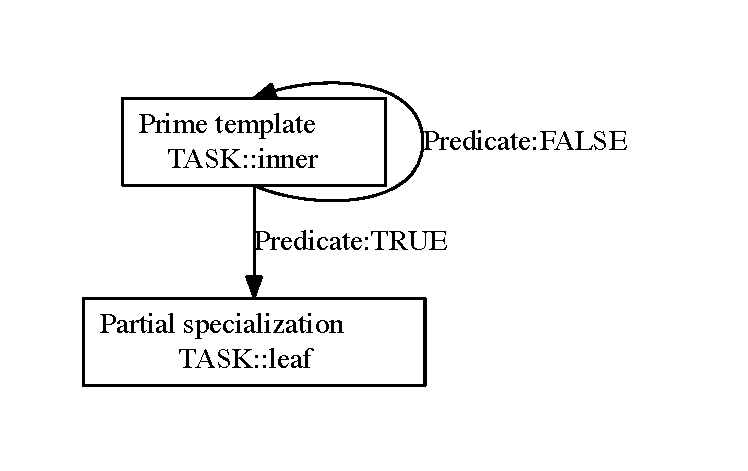
\includegraphics[width=3.5in]{../algo}
\caption{Instantiation process of TF\_hierarchy: The predicate is a template
class, which is evaluted using TASK' parameters.}\label{fig:hierarchy}
\end{figure}
%for sequoia's programming mode: 
%define recursive rules 
% for stream 's programming model:

\subsection{Adaption for TF\_pipeline}
To leverage TF\_pipeline, programmers have to provide a full
specialization template class for it. This is because TF\_pipeline
only synthesizes functions and executes them in order. It does not
know how to process the output. A full specialization of TF\_pipeline very defines
this behavior and is called at last. For \textit{langpipe} example,
line 2$\sim$21 is the case. Static entry at line 13 serves TF\_pipeline class. We spawn a thread to handle with the output of
precious last stage. Line 24$\sim$31 is a usage of TF\_pipeline with 4
standalone functions. All the stages including our customized one are
threads. It is noteworthy that each immediate stage \textit{e.g.}
\textit{translate$<$Frn2Spn$>$} has to follow type interfaces and
define dependences. In \textit{lang\_pipe} case, we utilize our ViewMT
despicted in Fig.~\ref{fig:view}. Asynchronous signals in ViewMTs provoke waiting
stages and are used to mimic data-flow diagram. Fig.~\ref{fig:viewmt} illustrates the scenario contains three
threads.

\begin{figure}[tp]
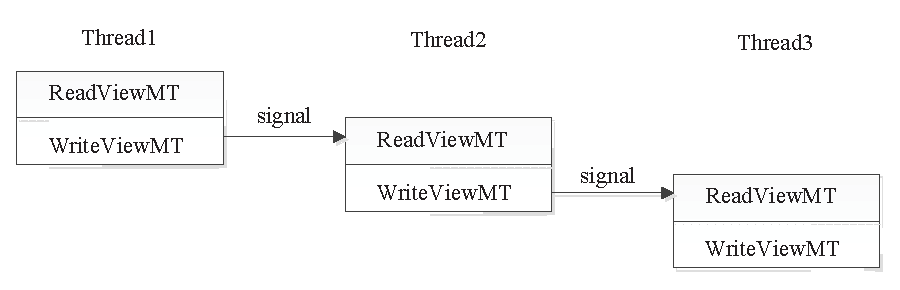
\includegraphics[width=3.1in]{../viewmt}
\caption{Pipeline process using ViewMTs: Access of a ViewMT is
  blocking until it is signaled. A stage sets its signal of WriteViewMT
after processing.}\label{fig:viewmt}
\end{figure}

%end of section.